\chapter[Metodologia]{Metodologia}

A metodologia utilizada será a pesquisa exploratória utilizando da revisão sistemática para encontrar a resposta à seguinte pergunta: “ Uma vez definido os indicadores das métricas, como criar uma interface de visualização da informação ? ”. O uso da pesquisa exploratória se deu por conta da baixa produção de artigos na área. A revisão sistemática é uma técnica criada na área da medicina que se difundiu para outras áreas de conhecimento por causa da produtividade que se ganha ao se deparar com um conjunto de artigos que não se sabe quais que se adequam ao conteúdo do autor. A revisão sistemática se dará em três etapas consecutivas: planejamento, execução e analise.


\begin{table}[http]
	\centering
	\caption{Cronograma TCC 1}
	\label{tab:cronograma}
	\begin{tabular}{ccccc}
		\hline
		\multicolumn{1}{|c|}{\textbf{Cronograma}}             & \multicolumn{1}{c|}{\textbf{Agosto}} & \multicolumn{1}{c|}{\textbf{Setembro}} & \multicolumn{1}{c|}{\textbf{Outubro}} & \multicolumn{1}{c|}{\textbf{Novembro}} \\ \hline
		\multicolumn{1}{|c|}{Realizar Pesquisa Bibliográfica} & \multicolumn{1}{c|}{X}              & \multicolumn{1}{c|}{X}              & \multicolumn{1}{c|}{X}             & \multicolumn{1}{c|}{X}              \\ \hline
		\multicolumn{1}{|c|}{Estudar o orgão}             & \multicolumn{1}{c|}{}               & \multicolumn{1}{c|}{X}              & \multicolumn{1}{c|}{X}             & \multicolumn{1}{c|}{}               \\ \hline
		\multicolumn{1}{|c|}{Propor Versão Inicial do dashboard}                & \multicolumn{1}{c|}{}               & \multicolumn{1}{c|}{}               & \multicolumn{1}{c|}{X}             & \multicolumn{1}{c|}{X}              \\ \hline
		\multicolumn{1}{l}{}                                  & \multicolumn{1}{l}{}                & \multicolumn{1}{l}{}                & \multicolumn{1}{l}{}               & \multicolumn{1}{l}{}                \\
		\multicolumn{1}{l}{}                                  & \multicolumn{1}{l}{}                & \multicolumn{1}{l}{}                & \multicolumn{1}{l}{}               & \multicolumn{1}{l}{}                \\
		\multicolumn{1}{l}{}                                  & \multicolumn{1}{l}{}                & \multicolumn{1}{l}{}                & \multicolumn{1}{l}{}               & \multicolumn{1}{l}{}               
	\end{tabular}
\end{table}

O plano metodológico consiste em duas fases iniciação e estudo da proposta. A primeira fase possui quatro atividades principais, são elas: Elaborar um roteiro de pesquisa, Pesquisar Referencias, Refinar Pesquisa e Catalogar material encontrado. Na atividade de elaboar um roteiro de pesquisa defini-se a string de busca e em quais bases serão pesquisados os materiais de referencia. A atividade de Pesquisar referencias como o próprio nome ja sugere envolve a pesquisa da string de busca nas bases selecionadas. Refinar pesquisa envolve elaborar uma nova string de busca que contenha termos mais especificos e que aumente a quantidade de arquivos referentes ao tema. Catalogar material é uma atividade focada em guardar os materiais encontrados colocando uma tag referente ao tema a que o artigo se refere e uma breve descrição sobre o que era mais importante. 
\\A Segunda fase consiste em estudar o cenario em que será colocado a dashboard para que se possa entender quais as necessidades e os requisitos para implantação. Esta fase está dividida em três momentos: planejar,  executar e checar. Durante o momento de planejar tem-se como principais atividades analisar o problema onde há um maior entendimento do contexto no qual será elaborado a solução. A segunda atividade é elaborar solução em que é esperado que ao fim dessa atividade exista um esboço do que será a solução final. No segundo momento implementa-se a solução e no terceiro momento acontece a validação dessa solução.
\graphicspath{{figuras/}}
\begin{figure}
\centering
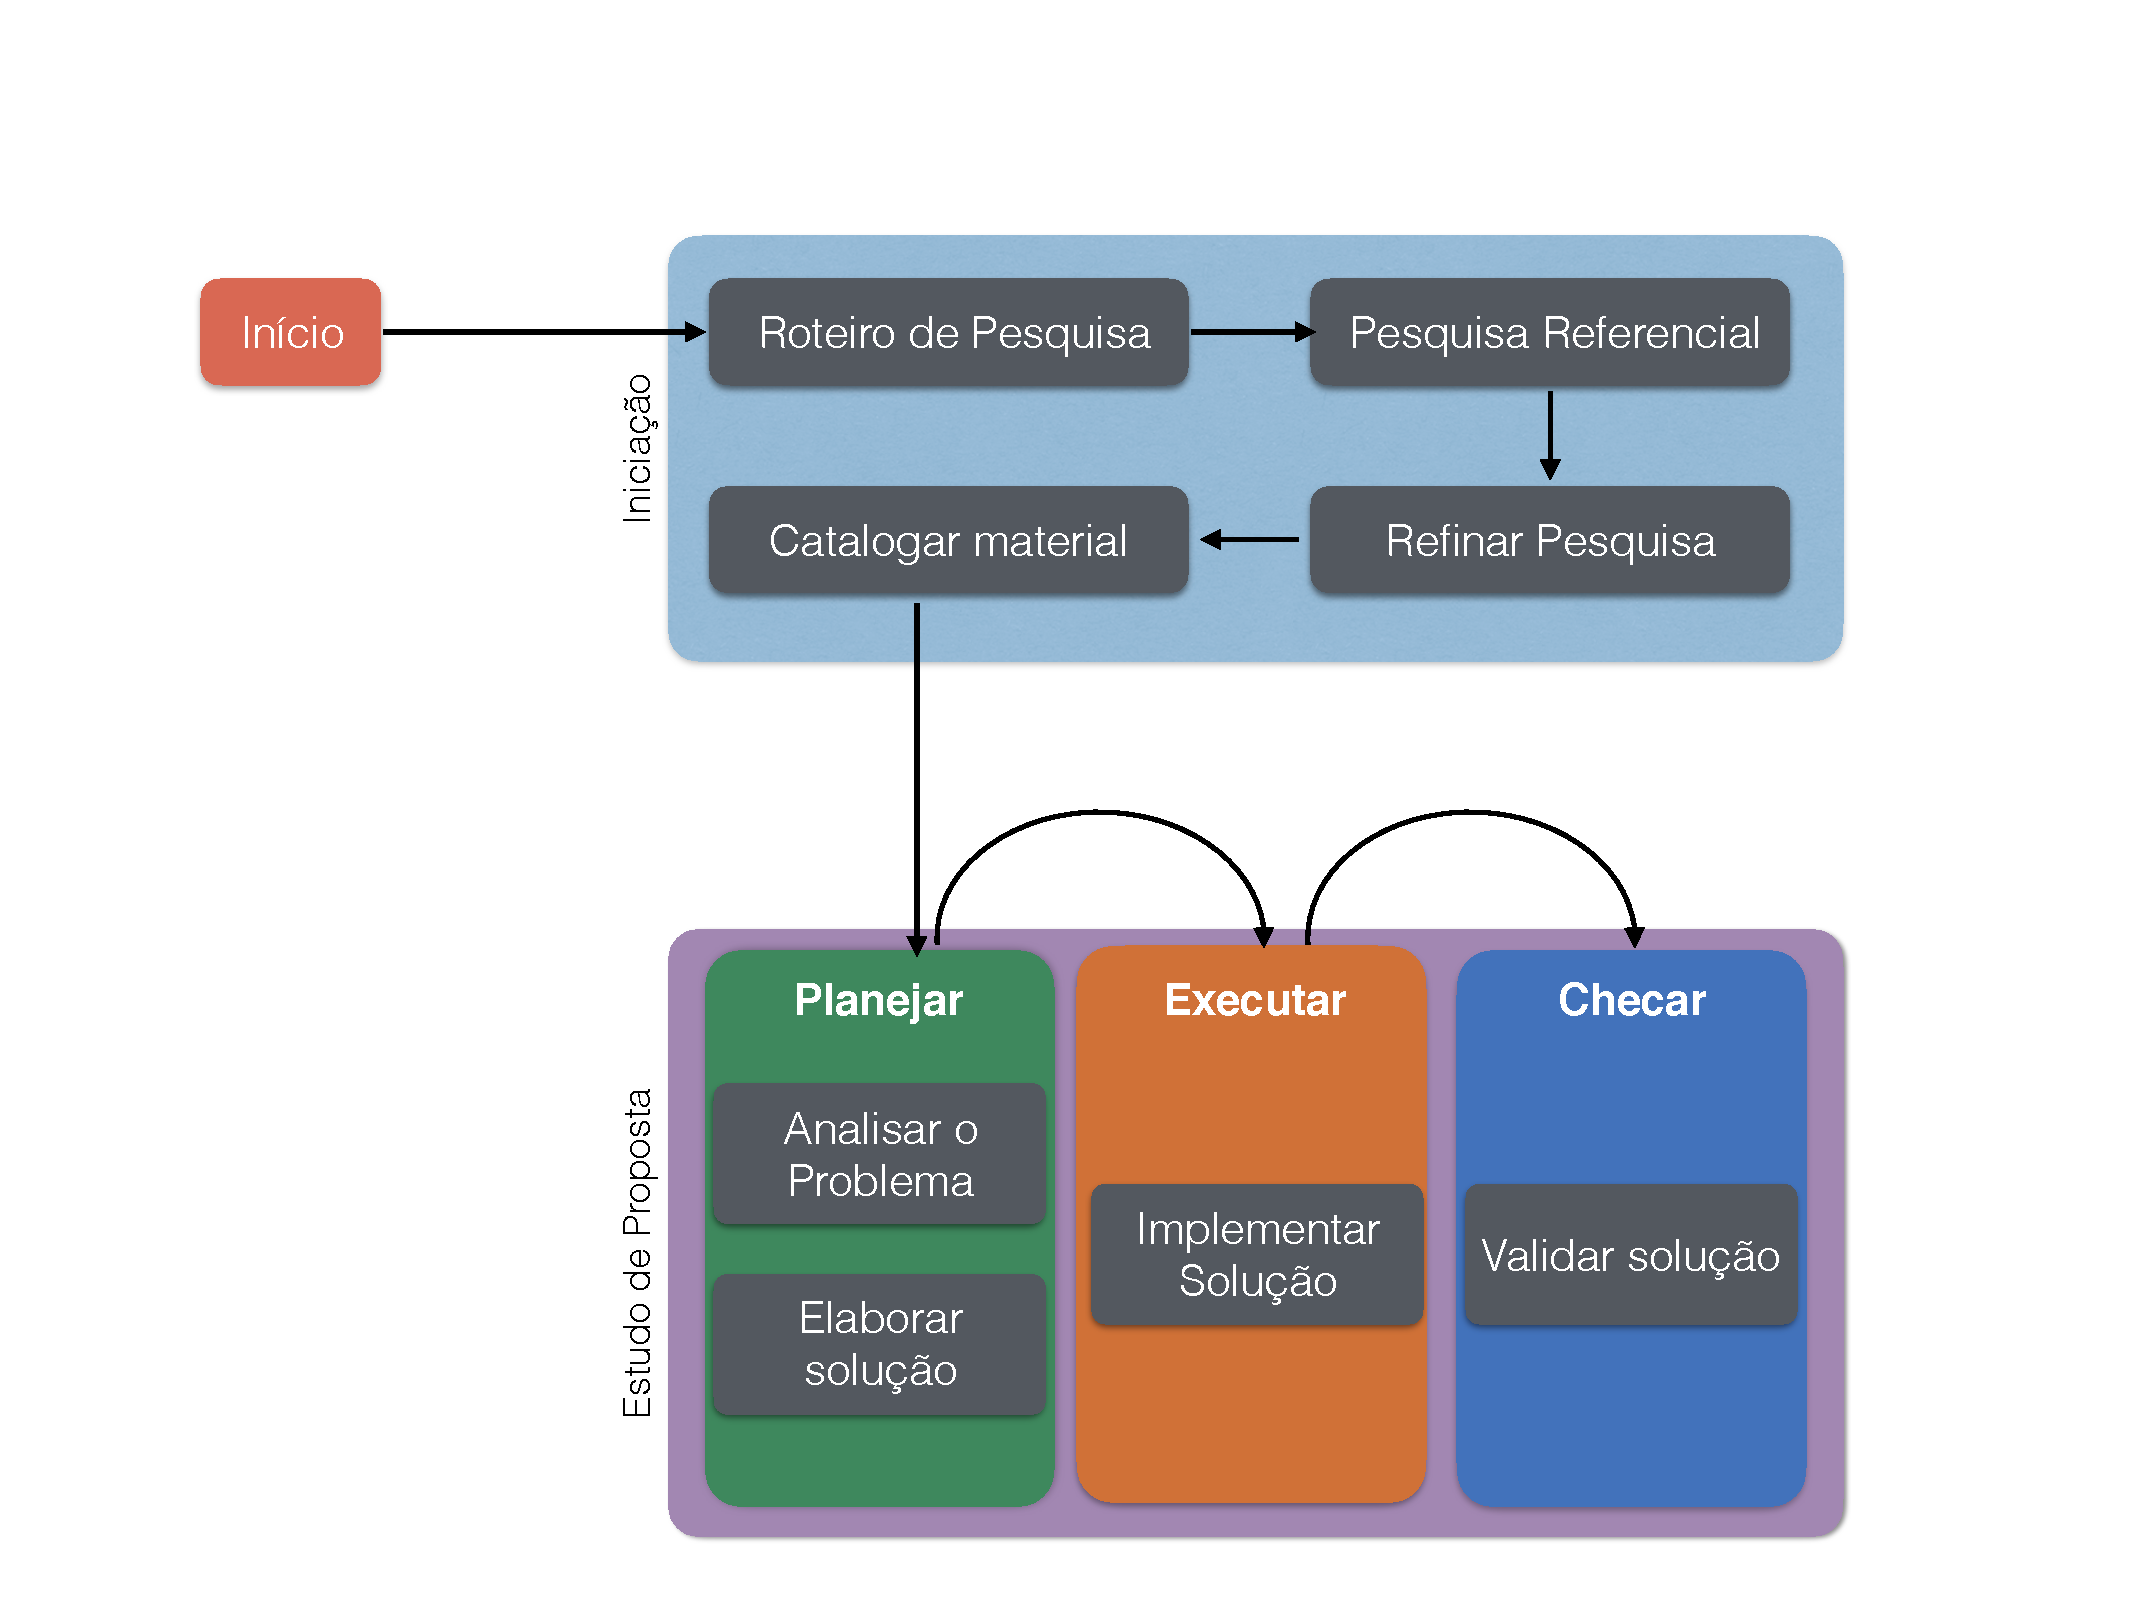
\includegraphics[scale=0.40]{TCCMetodologia}
\caption{Plano de Pesquisa}
\label{Rotulo}
\end{figure}
